\documentclass[tikz,border=2pt]{standalone}
\renewcommand{\familydefault}{\sfdefault}
\usetikzlibrary{arrows.meta,calc,positioning}
\tikzset{every picture/.style={line width=1pt, >=Stealth},
         hl/.style={fill=black, fill opacity=0.12, text opacity=1}}
\begin{document}
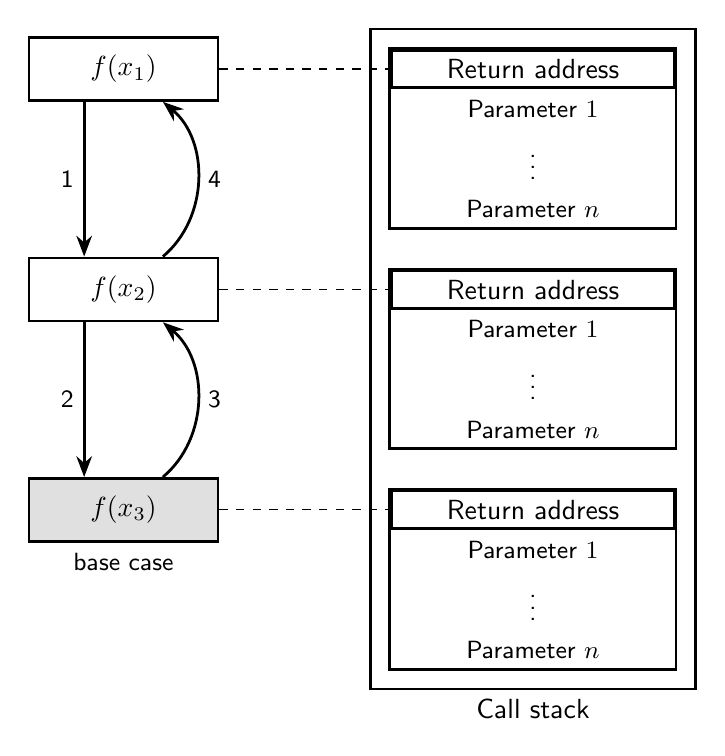
\begin{tikzpicture}[call/.style={draw, minimum width=2.4cm, minimum height=0.8cm},
    field/.style={minimum width=3.6cm, minimum height=0.45cm, font=\small}]
  % Calls (1, 2) go down to the base case; returns (3, 4) come back up.
  \foreach \k in {1, 2, 3} \node[call] (f\k) at (0, -2.8*\k + 2.8) {$f(x_\k)$};
  \node[call, hl] at (f3) {};
  \node[below, font=\small] at (f3.south) {base case};
  \draw[->] ([xshift=-0.5cm]f1.south) -- node[left, font=\small] {1} ([xshift=-0.5cm]f2.north);
  \draw[->] ([xshift=-0.5cm]f2.south) -- node[left, font=\small] {2} ([xshift=-0.5cm]f3.north);
  \draw[->] ([xshift=0.5cm]f3.north) to[bend right=50] node[right, font=\small] {3} ([xshift=0.5cm]f2.south);
  \draw[->] ([xshift=0.5cm]f2.north) to[bend right=50] node[right, font=\small] {4} ([xshift=0.5cm]f1.south);

  % One stack frame per call, each holding a return address and the parameters.
  \foreach \k in {1, 2, 3} {
    \node[field, draw, font=\normalsize] (ret\k) at (5.2, -2.8*\k + 2.8) {Return address};
    \node[field, below=0pt of ret\k] (p\k) {Parameter $1$};
    \node[field, below=0pt of p\k] (d\k) {$\vdots$};
    \node[field, below=0pt of d\k] (n\k) {Parameter $n$};
    \draw (ret\k.north west) rectangle (n\k.south east);
    \draw[thin, dashed] (f\k.east) -- (ret\k.west);
  }
  \draw ([shift={(-0.25, 0.25)}]ret1.north west) rectangle ([shift={(0.25, -0.25)}]n3.south east);
  \node[below] at ([yshift=-0.25cm]n3.south) {Call stack};
\end{tikzpicture}
\end{document}
